\chapter{Results}\label{sec:results}
To verify both the correctness and the gain in terms of performance of the new implementation of the bistable simulation engine many circuits has been tested both with CPU and GPU. The characteristics of the architectures used to run the simulations are shown in the table \ref{tab:architectures}. The CPU used for the execution of the parts of the new code that does not run on the GPU is the same CPU that has bee used for the execution of the other simulations.

\begin{table}[h!tb]
   \centering \caption{CPU simulation Profiling}
   \label{tab:architectures}
   \vskip 0.2cm
   %%
   \scalebox{0.90}{
	    %% The {|c|c|c|c|c|} define the number of columns.
	    %% c means centered
	    %% | defines a vertical line between two columns 
	    \begin{tabular}{|c|c|c|}
	      \hline
	      Type & CPU& GPU \\
	      \hline
	      Model& Xeon E5345 & Tesla C1060 \\
	      \hline
	      Cores & 8 & 240  \\
	      \hline
	      Memory & 8 Gb & 4 Gb  \\
	      \hline
	      Freq & 2 Ghz & 1,3 Ghz  \\
	      \hline
	    \end{tabular}
	 }
 \end{table}

As already said in \ref{sec:cpu_algorithm} the parameters that mainly affect simulation time are the number of inputs, which define the samples for the simulation, and the number of cells. We choose a wide range of circuit in order to get a good estimation of the speedup with different values of both samples and number of cells. The tested circuits have from 2 to 6  inputs and froma a minimum of 30 cells to a maximum of 35.000 cells. \newline
During the optimization we focused on the parallelization of the computation of new polarizations, so we expected to see lower execution times with resepct to the cpu with the increasing of the number of cells. This hypothesis has been confirmed by the results of the simulations.

\begin{figure}
\centering
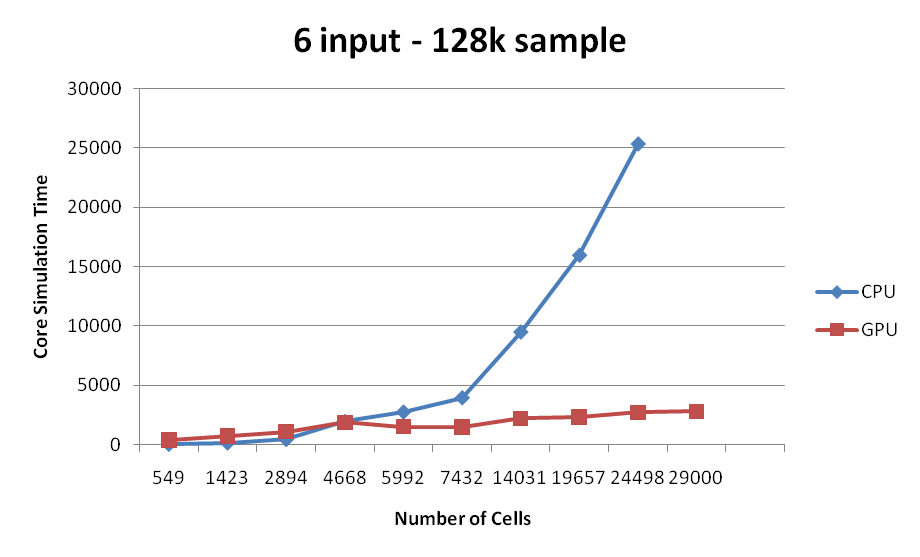
\includegraphics[scale=0.6]{img/graph5_core.png}
\caption{Comparison of the core simulation time between CPU and GPU}
\label{img:graph5}
\end{figure}

Figure \ref{img:graph5} shows the comparison between the execution time of the CPU simulation and the one on the GPU, on the vertical axis there is the core simulation time which is the time spent to convert original structures to arrays,to perform the coloring and to run the simulation.\newline
The simulation output obtained with the new implementation and the previous one are the same and are illustrated in figure \ref{img:result}. The difference of the output value in the initial samples are due to the delay of the circuit illustrated in \ref{sec:clock}. This is the output of a circuit with 3 inputs.

\begin{figure} [h!]
\centering
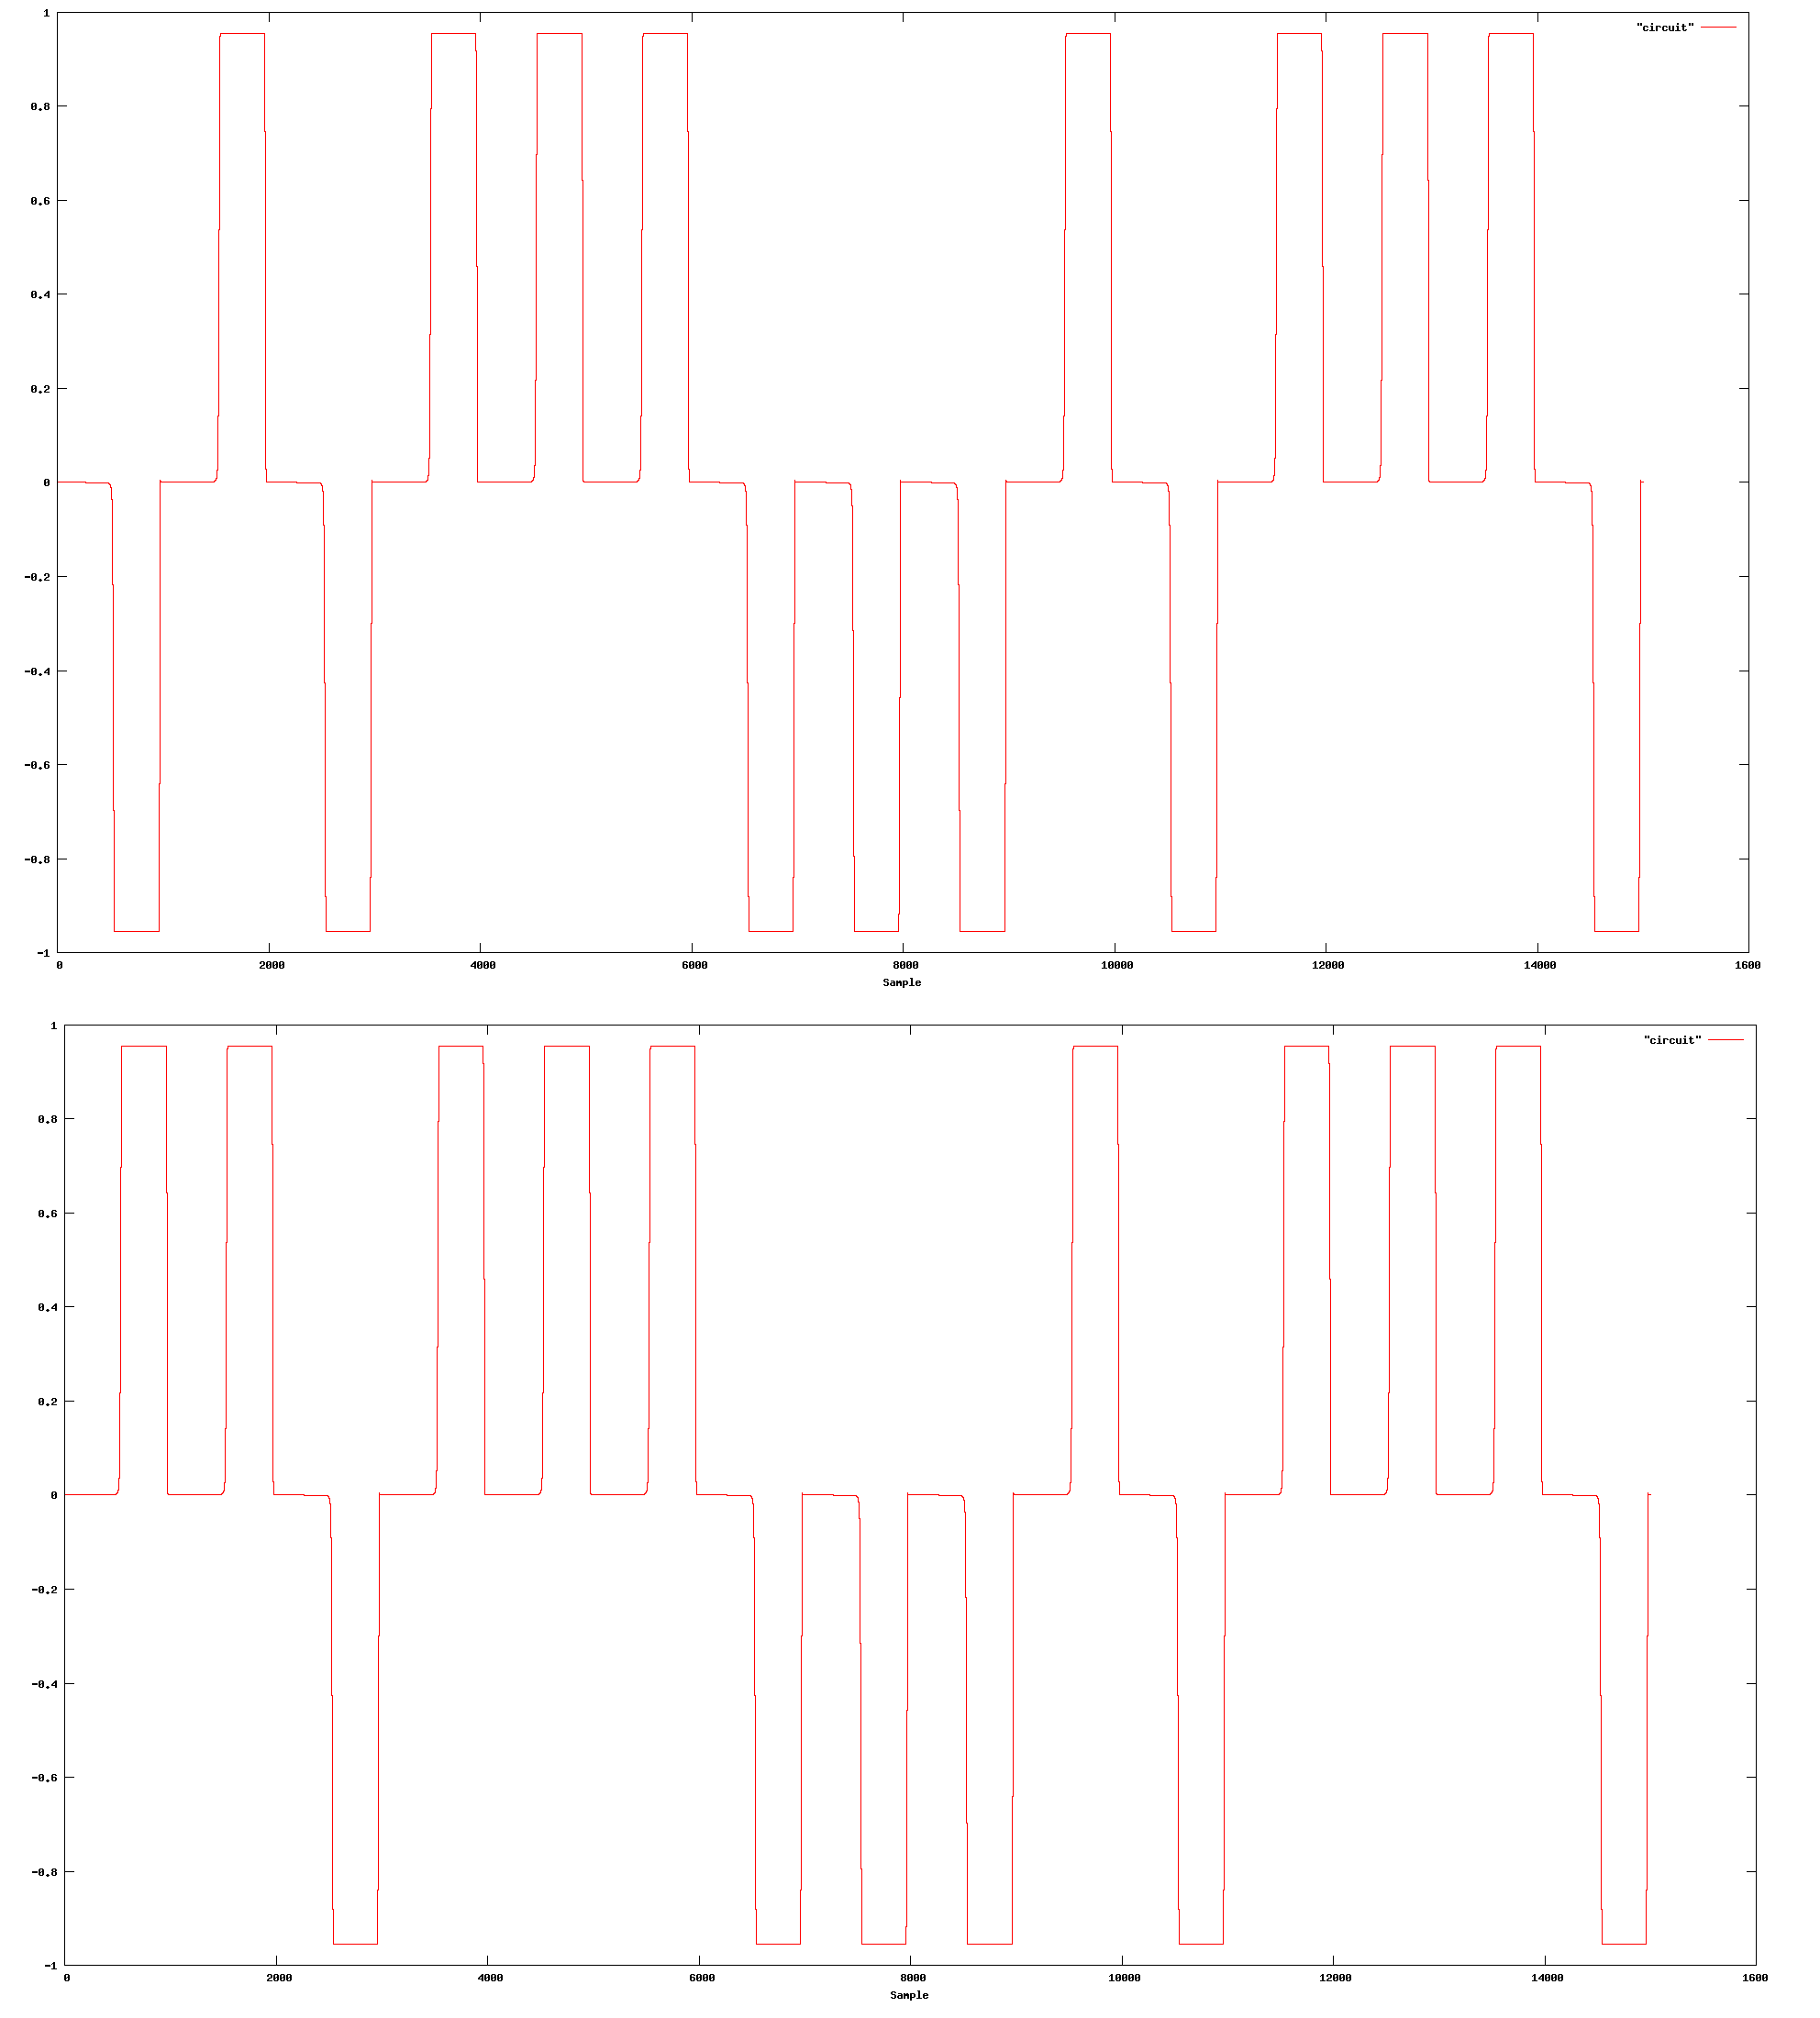
\includegraphics[scale=0.2]{img/result.png}
\label{img:result}
\end{figure}

As expected the initial speedup is lower than one and it grows with the number of cells in the circuit. Over a certain number of cells the speedup meets an upper bound. This limitation is due to the fact that the GPU can execute in parallel much less threads than the actual number of cells, for this reason the GPU is forced to serialize the execution of some threads. This is an intrinsic limitation of the architecture use for the simulation, not derived by the implementation. Using a GPU which allows more parallel threads the upper bound will be raised. The average speedup on the tested circuits with 4 inputs is of 2,2. The minimum speedup, which corresponds to the circuit with less cells is of 0,006 and the maximum is of 8,7. Increasing the number of samples of the simulation the upper limit of the speedup is increased because the fraction of the entire code that has been accelerated is executed more times.

\begin{figure}
\centering
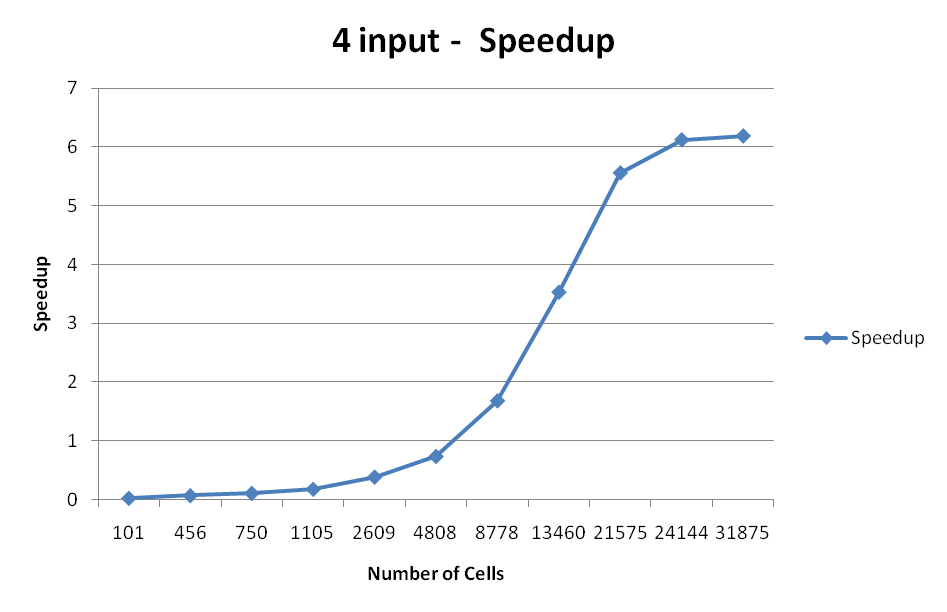
\includegraphics[scale=0.6]{img/speed.png}
\label{img:speed}
\end{figure}

Figures \ref{img:result1}, \ref{img:result2}, \ref{img:result3}, \ref{img:result4}, \ref{img:result5}, shows the results of all the simulations. Figure \ref{img:speed} shows the speedup of the new implementation on the previous one. As expected all the charts shows that the GPU execution time is less subject to the number of cells in the circuit. The different values of the upper bound of the speedup is due to the difference in the simulated circuits. Especially in figure \ref{img:result1} the speedup of the last circuit simulated is lower than the previous one, this is due to the fact that the particular design of this circuit converged in less iterations.